%%%%%%%%%%%%%%%%%%%%%%%%%%%%%%%%%%%%%%%%%
% University/School Laboratory Report
% LaTeX Template
% Version 4.0 (March 21, 2022)
%
% This template originates from:
% https://www.LaTeXTemplates.com
%
%%%%%%%%%%%%%%%%%%%%%%%%%%%%%%%%%%%%%%%%%

%----------------------------------------------------------------------------------------
%	PACKAGES AND DOCUMENT CONFIGURATIONS
%----------------------------------------------------------------------------------------

\documentclass[
	a4paper, % Paper size, specify a4paper (A4) or letterpaper (US letter)
	10pt, % Default font size, specify 10pt, 11pt or 12pt
]{CSUniSchoolLabReport}

\addbibresource{sample.bib} % Bibliography file (located in the same folder as the template)

%----------------------------------------------------------------------------------------
%	REPORT INFORMATION
%----------------------------------------------------------------------------------------

\title{Report 5: Quantum Monte Carlo} % Report title
\subtitle{Git: https://github.com/simonblaue/MCP-Ex5.git}

\author{Simon \textsc{Blaue}} % Author name(s), add additional authors like: '\& James \textsc{Smith}'


\date{\today} % Date of the report

%----------------------------------------------------------------------------------------

\begin{document}

\maketitle % Insert the title, author and date using the information specified above

\vspace*{40px}

\begin{tabular}{l r}
	Universität Göttingen \\ % Date the experiment was performed
	Faculty of Physics \\
	Instructor: Prof. Dr. S. Schumann \\
	Tutors: Dr. E. Bothmann, M. Knobbe \\ % Partner names
\end{tabular}


% If you need to include an abstract, uncomment the lines below
%\begin{abstract}
%	Abstract text
%\end{abstract}

\newpage
%----------------------------------------------------------------------------------------
%	CONTENT
%----------------------------------------------------------------------------------------
% \headtopline
% \headsepline

\ohead{\pagemark}
\automark{subsection}

\section{Variational Monte Carlo simulation of a Helium atom}

\subsection{Investigate stepsize $s$}

\begin{figure}[H]
	\begin{subfigure}[b]{0.49\textwidth}
		\centering
		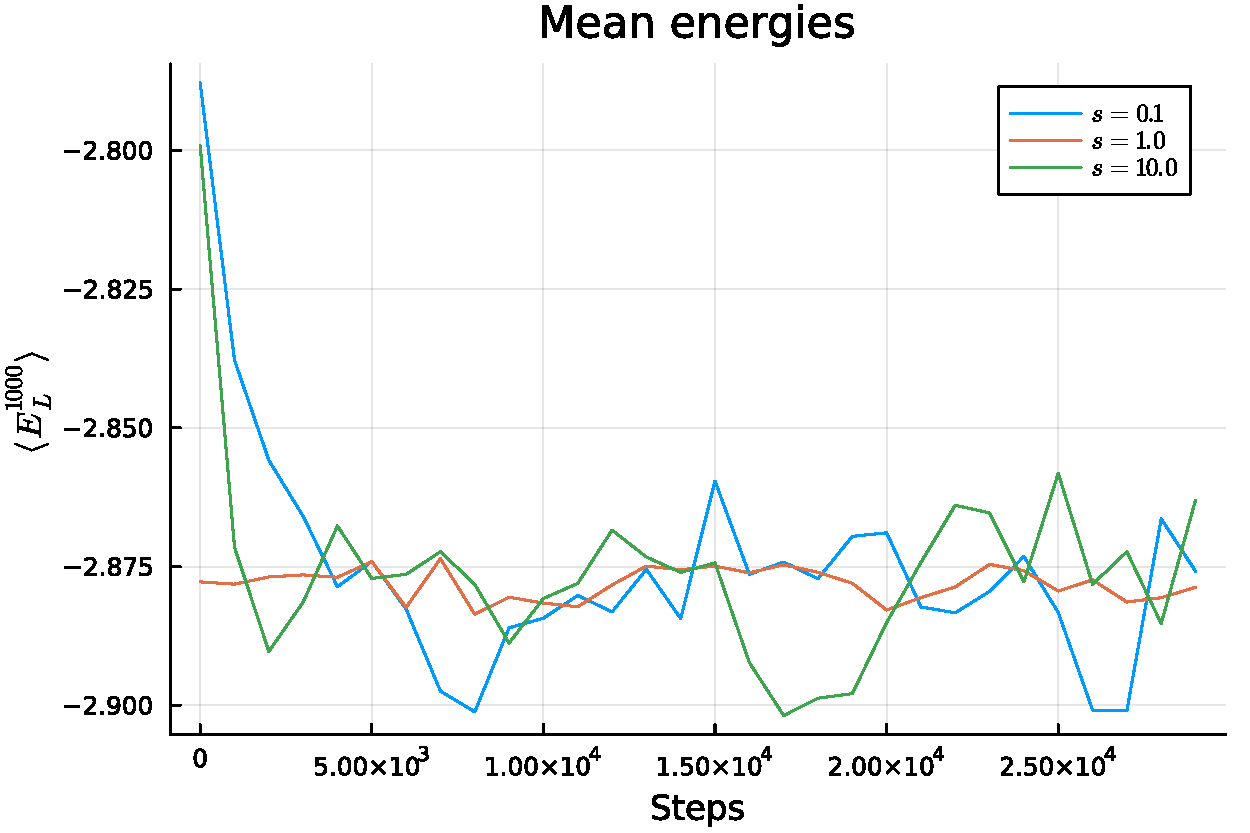
\includegraphics[width=\textwidth]{../saves/task1a.energies.pdf}
		\caption{Energies}
		% \label{fig:three sin x}
	\end{subfigure}
	\hfill
	\begin{subfigure}[b]{0.49\textwidth}
		\centering
		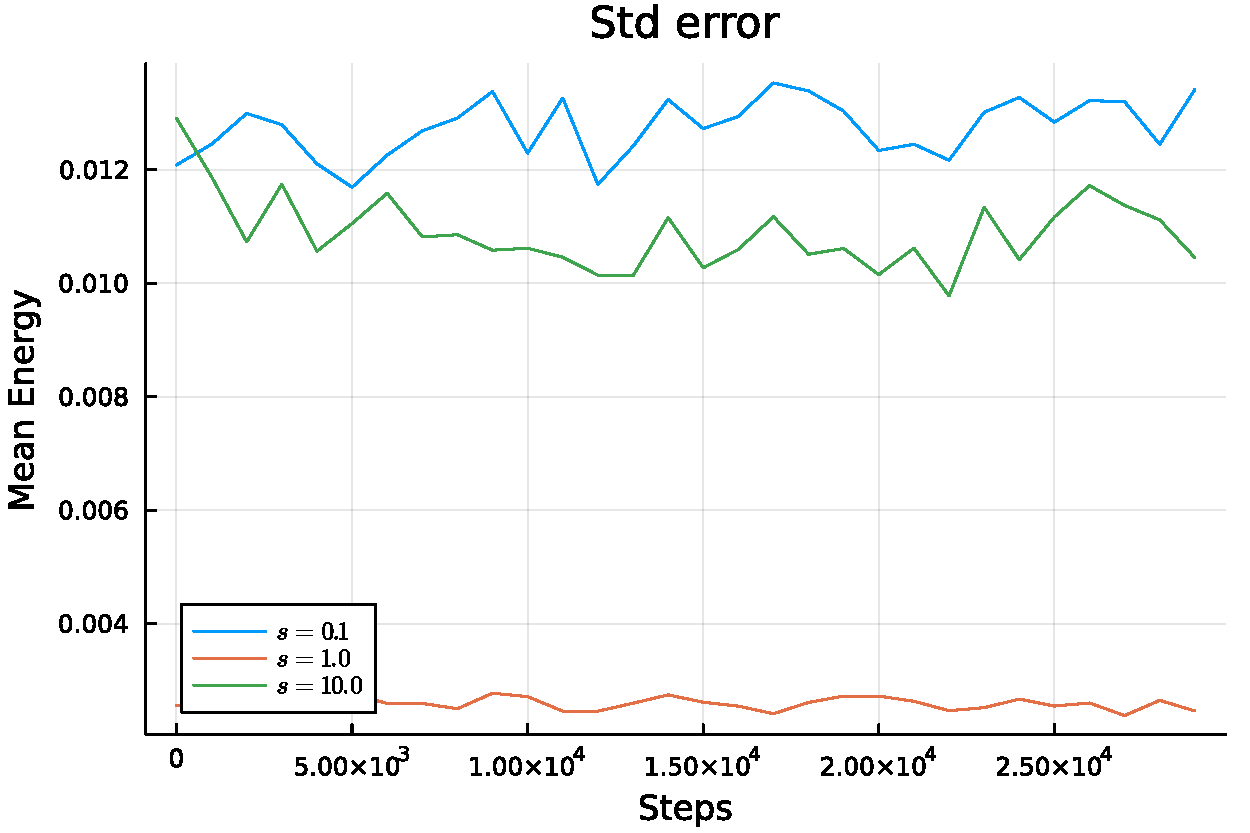
\includegraphics[width=\textwidth]{../saves/task1a.stds.pdf}
		\caption{Stds}
		% \label{fig:three sin x}
	\end{subfigure}
\end{figure}

\subsection{Approximating equilibration time}

\begin{figure}[H]
	\begin{subfigure}[b]{0.49\textwidth}
		\centering
		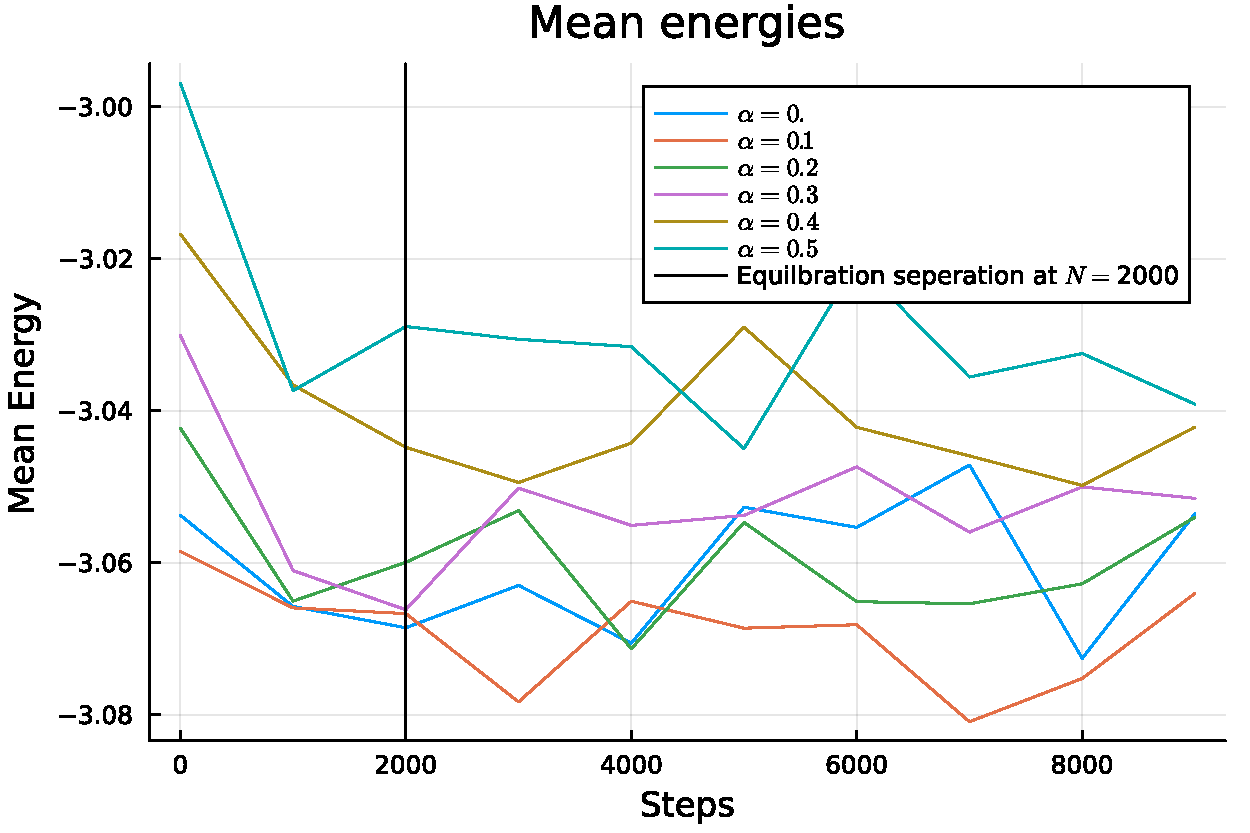
\includegraphics[width=\textwidth]{../saves/task1b.energies.pdf}
		\caption{Energies}
		% \label{fig:three sin x}
	\end{subfigure}
	\hfill
	\begin{subfigure}[b]{0.49\textwidth}
		\centering
		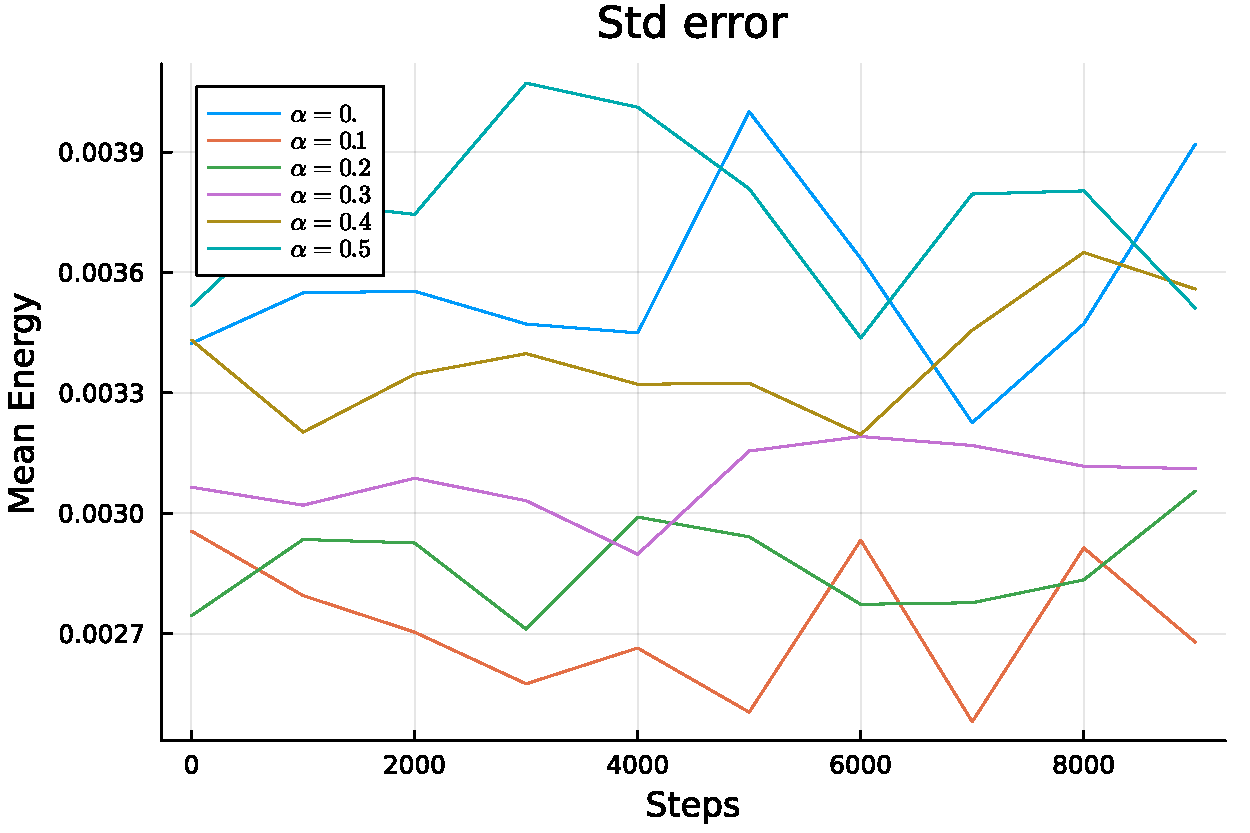
\includegraphics[width=\textwidth]{../saves/task1b.stds.pdf}
		\caption{Stds}
		% \label{fig:three sin x}
	\end{subfigure}
\end{figure}

\subsection{Investigate variational parameter $\alpha$}

\begin{figure}[H]
	\begin{subfigure}[b]{0.49\textwidth}
		\centering
		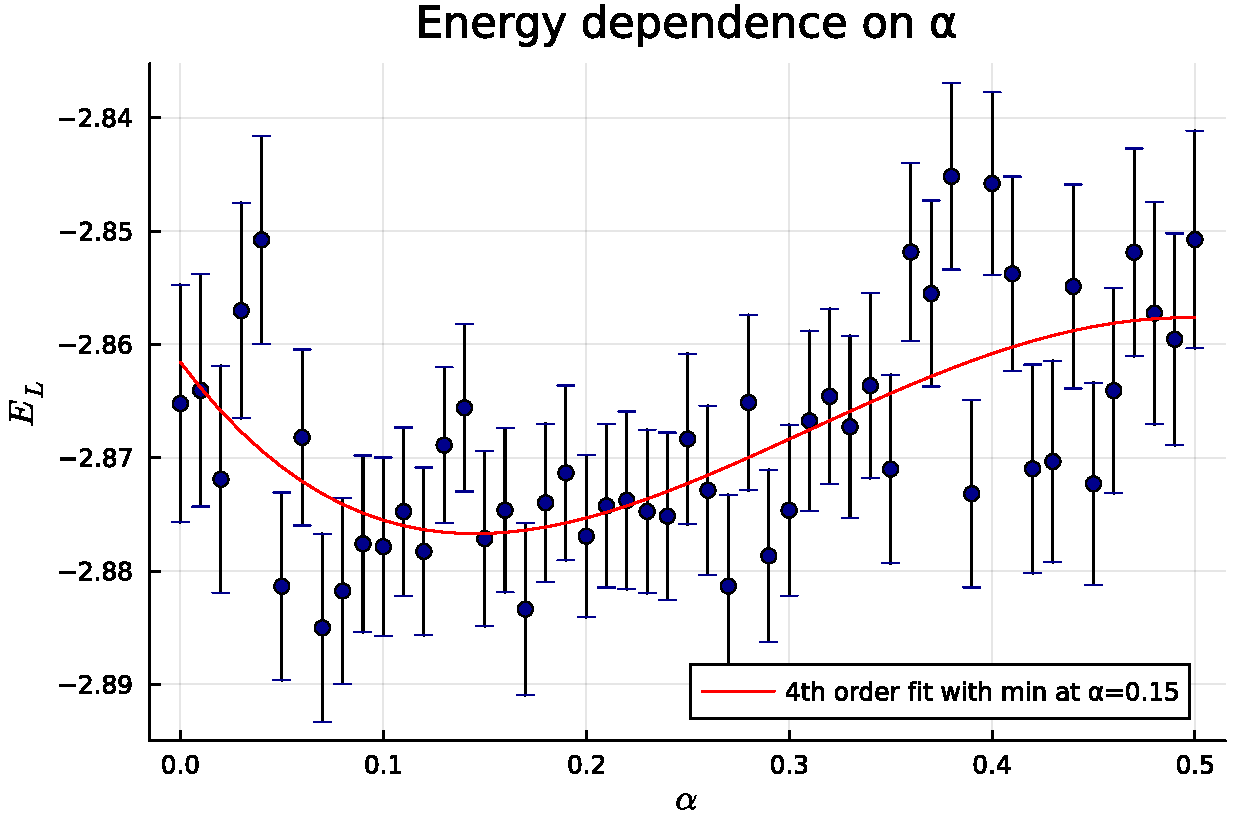
\includegraphics[width=\textwidth]{../saves/task1c.avEnergies.pdf}
		\caption{Energies}
		% \label{fig:three sin x}
	\end{subfigure}
	\hfill
	\begin{subfigure}[b]{0.49\textwidth}
		\centering
		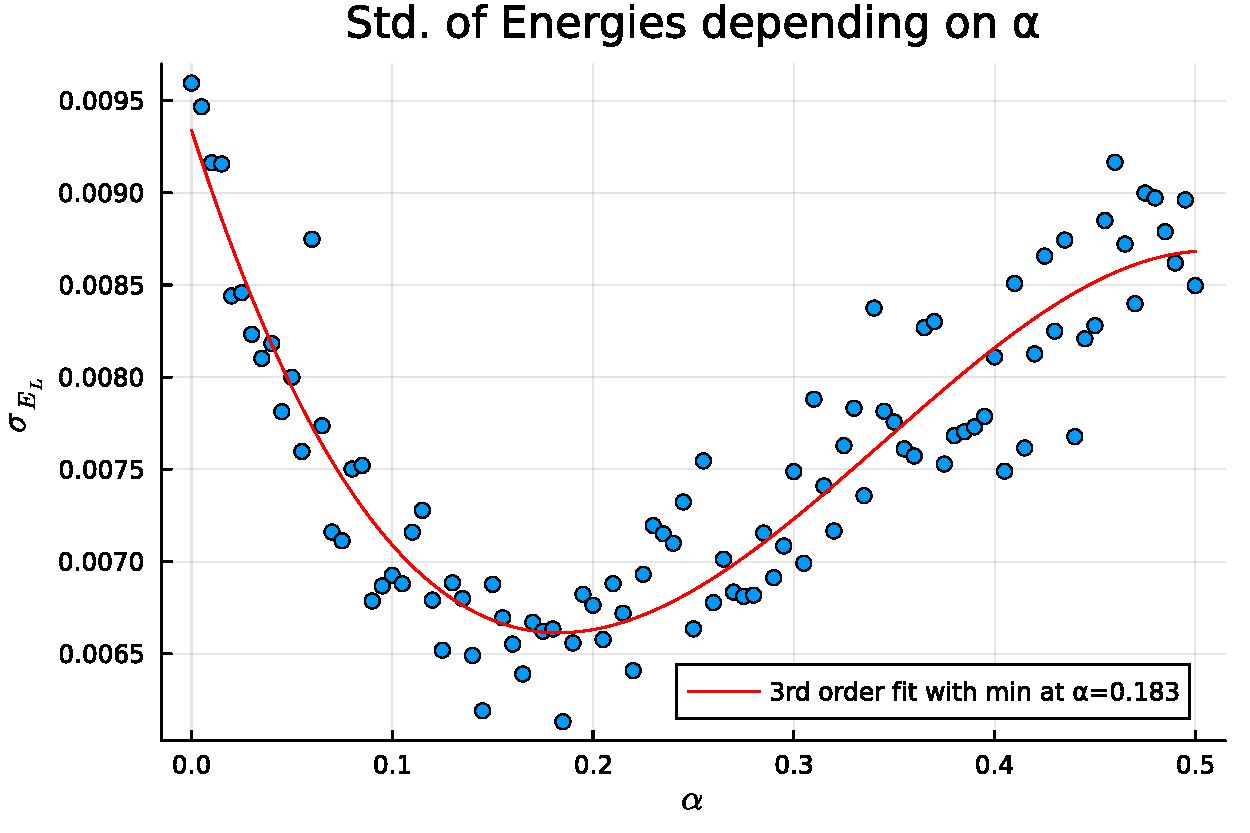
\includegraphics[width=\textwidth]{../saves/task1c.avStd.pdf}
		\caption{Stds}
		% \label{fig:three sin x}
	\end{subfigure}
\end{figure}

\subsection{Investigate variational Parameter $\kappa$}

\begin{figure}[H]
	\begin{subfigure}[b]{0.49\textwidth}
		\centering
		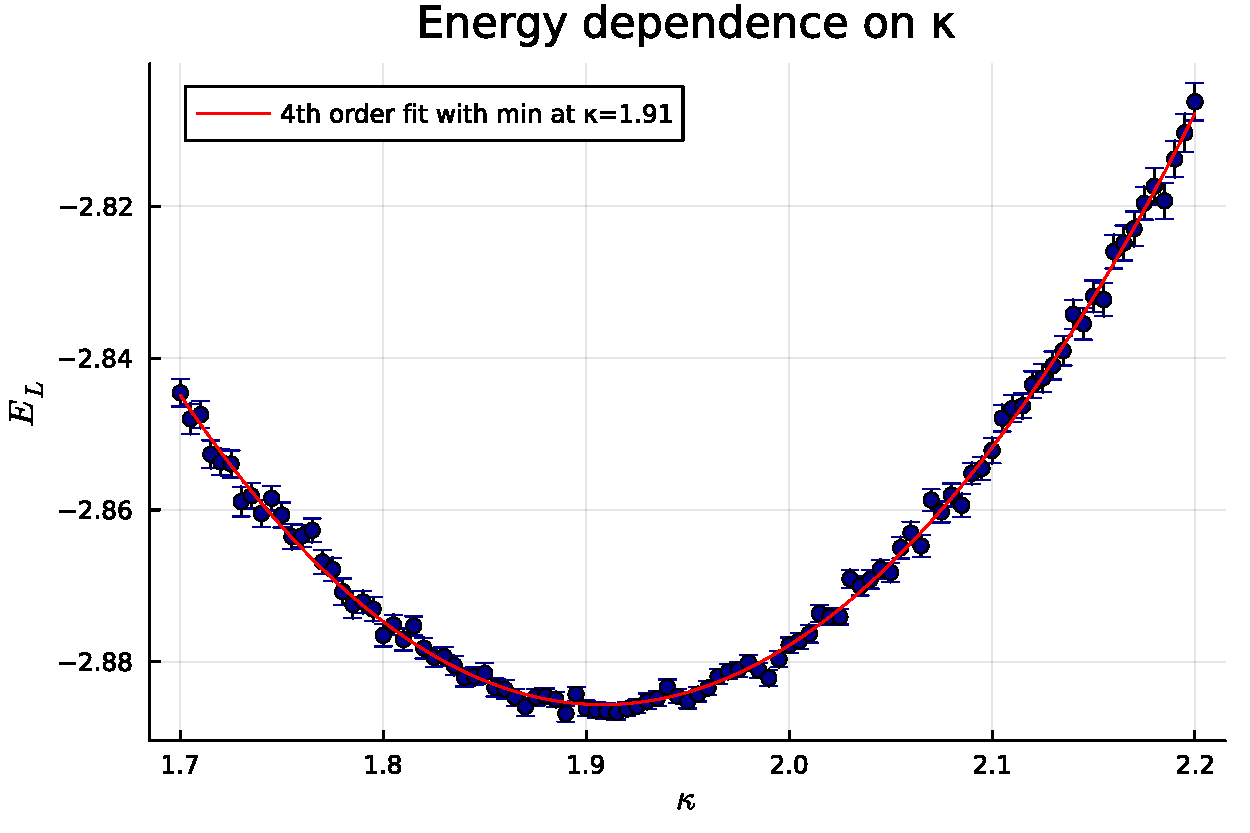
\includegraphics[width=\textwidth]{../saves/task1d.avEnergies.pdf}
		\caption{Energies}
		% \label{fig:three sin x}
	\end{subfigure}
	\hfill
	\begin{subfigure}[b]{0.49\textwidth}
		\centering
		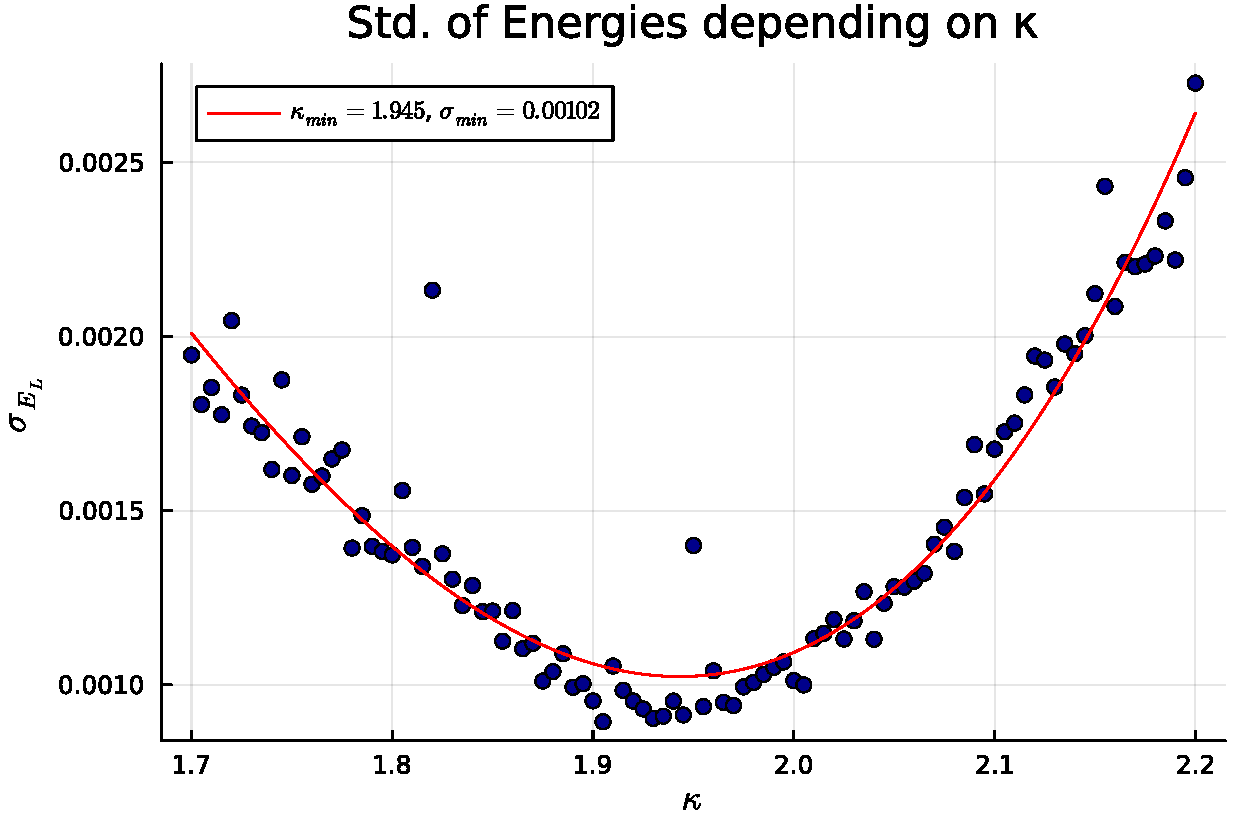
\includegraphics[width=\textwidth]{../saves/task1d.avStd.pdf}
		\caption{Stds}
		% \label{fig:three sin x}
	\end{subfigure}
\end{figure}

\subsection{Optimizing parameters $\alpha$, $\beta$ and $\kappa$}

Strange stuff happens, optimizing for minimal energie leads to a lower energie as with given params, but higher std...

\section{Variational Monte Carlo with Fokker-Plank support}

\begin{figure}[H]
	\begin{subfigure}[b]{0.49\textwidth}
		\centering
		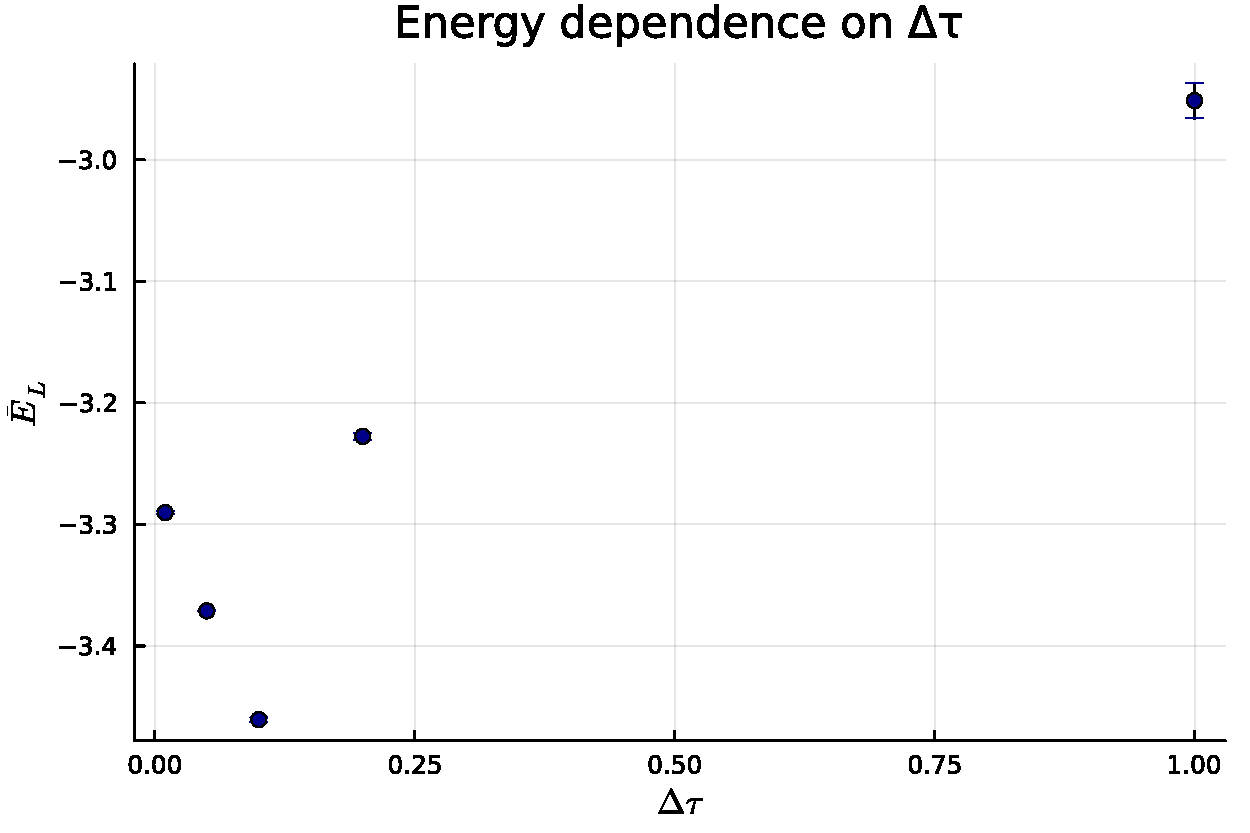
\includegraphics[width=\textwidth]{../saves/task1g.avEnergies.pdf}
		\caption{Energies}
		% \label{fig:three sin x}
	\end{subfigure}
	\hfill
	\begin{subfigure}[b]{0.49\textwidth}
		\centering
		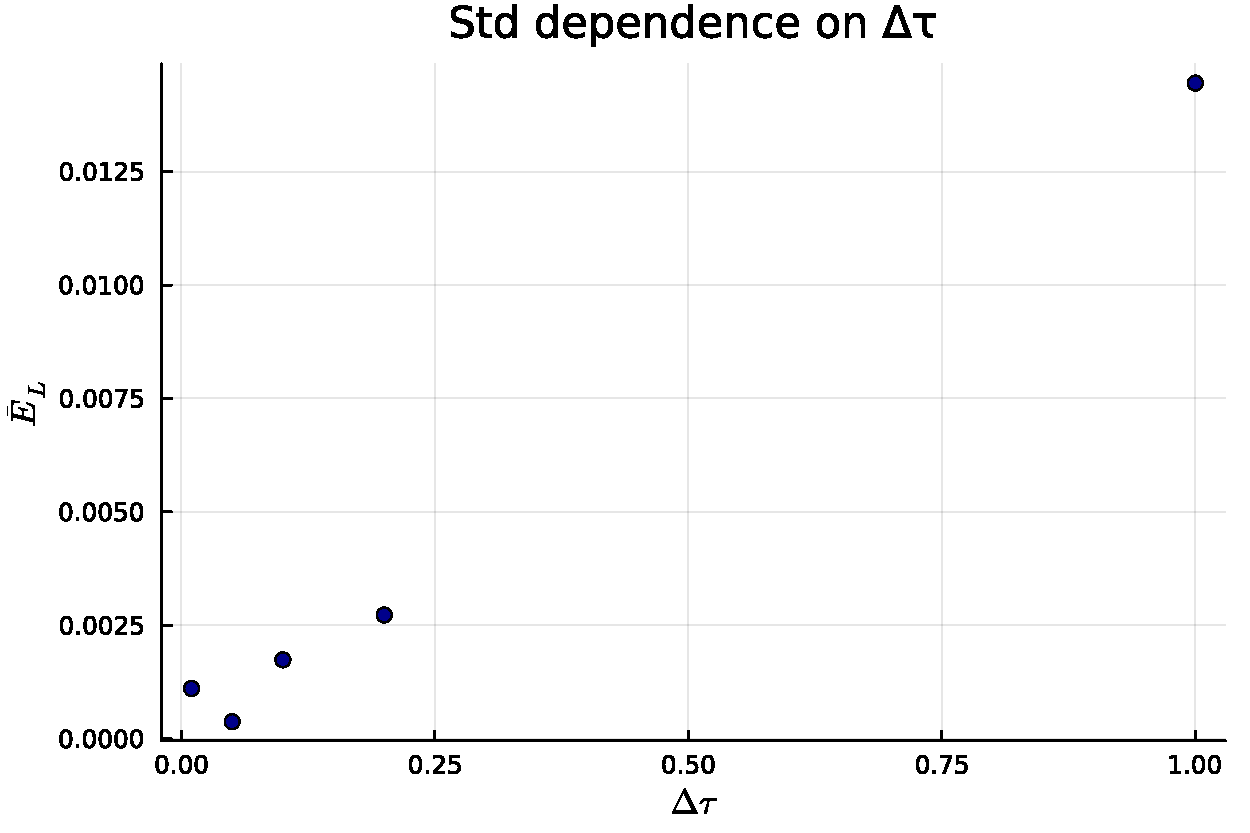
\includegraphics[width=\textwidth]{../saves/task1g.avStd.pdf}
		\caption{Stds}
		% \label{fig:three sin x}
	\end{subfigure}
\end{figure}

\subsection{Quantum force}

\subsection{Investigate variational parameter $\Delta\tau$}

\subsection{Electron density}

\section{Diffusion Monte Carlo simulation of a Helium atom}

\section{Feynman Path Integral Quantum Mechanics}

%----------------------------------------------------------------------------------------
%	DISCUSSION
%----------------------------------------------------------------------------------------

% \section{Discussion}



%----------------------------------------------------------------------------------------
%	BIBLIOGRAPHY
%----------------------------------------------------------------------------------------
\newpage

\printbibliography % Output the bibliography

%----------------------------------------------------------------------------------------

\end{document}